% !TEX TS-program = pdfLaTeX+shellescape
% !TEX encoding = UTF-8 Unicode

\documentclass[class=beamer,tikz]{standalone}
\setbeamertemplate{navigation symbols}{} % For delete the navigation symbols
\usepackage{pgfplots}
\pgfplotsset{compat=1.17}

\begin{document}
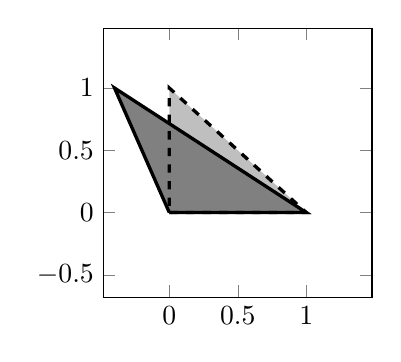
\begin{tikzpicture}[baseline]
\begin{axis}[
scale=0.6, % scale
xmin=-0.48,xmax=1.48,ymin=-0.68,ymax=1.48, % range of plot
legend style={at={(axis cs: 1,0)}, anchor=south east}, % position of legends
unit vector ratio = {1,1}, % aspect ratio
axis lines = box, % middle or box
%axis x line = bottom, % top, middle, bottom, none: axis x line* = ... removes arrow heads
%axis y line = left, % left, center, right, none: axis y line* = ... removes arrow heads
%xlabel = {$x$}, ylabel = {$y$}, % axis labels 
]
\coordinate (A) at (axis cs:0,0);
\coordinate (B) at (axis cs:1,0);
\coordinate (C) at (axis cs:0,1);
\coordinate (C') at (axis cs:-0.4,1);
\fill[gray!50] (A) -- (B) -- (C) -- (A);
\fill[gray] (A) -- (B) -- (C') -- (A);
\draw[very thick,dashed] (A) -- (B) -- (C) -- (A);
\draw[very thick] (A) -- (B) -- (C') -- (A);
\end{axis}
\end{tikzpicture}
\end{document}